\model{Stack Diagrams}

Each function has its own area of memory to store parameters and other variables.
When a function is invoked, C++ allocates this memory on the \emph{call stack}.
For convenience, we draw ``stack'' diagrams upside down.

\begin{center}
\includegraphics[height=3in]{stack-rings1.png}
\hspace{1em}
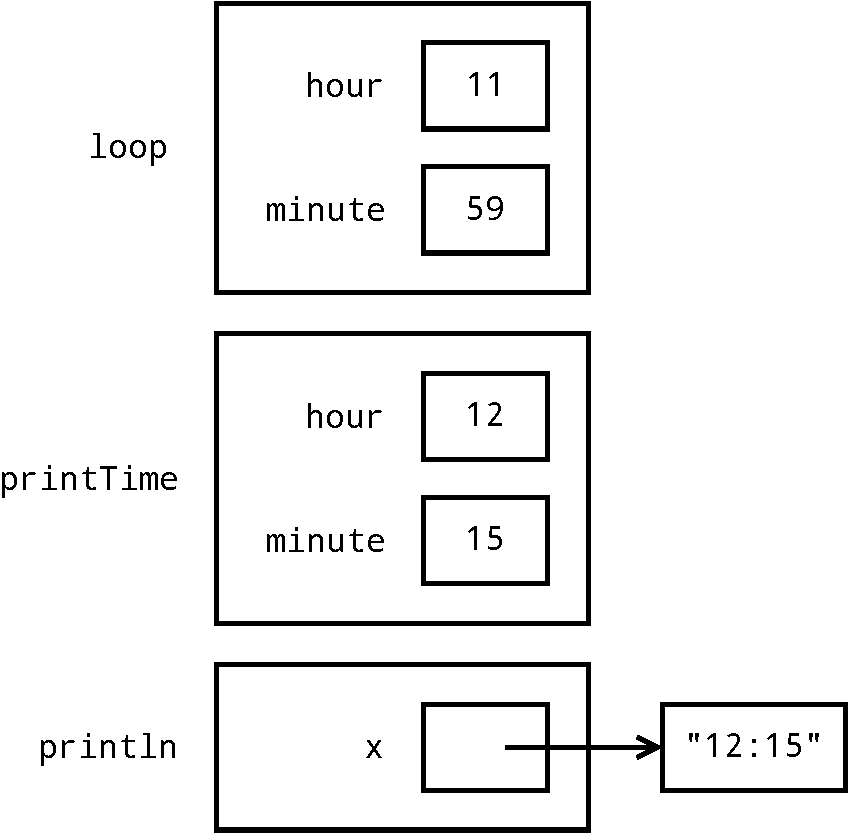
\includegraphics[height=3in]{stack1_loop-crop.pdf}
\end{center}

% \begin{center}
% Note: The signature for \java{System.out.println} is ~\java{public void println(String x)}.
% \end{center}

\begin{javalst}
void printTime(int hour, int minute) {
    Serial.println(String(hour) + ":" + String(minute));
}

void loop() {
    int hour = 11;
    int minute = 59;
    printTime(12, 15);

    while(true) {
    }
}
\end{javalst}



\Q Based on the diagram, how many functions does the program call? \ans{Three}
\vspace{1ex}


\Q Based on the diagram, how many variables does the program have? \ans{Five}
\vspace{1ex}


\Q How is it possible that two variables with the same name can have different values?

\begin{answer}
Each method declares its own variables.
Because they are stored in different memory locations, the values are independent from other methods.
\end{answer}

\newpage

\model{Tossing in loops and global variables}

The program below has a global variable (\java{ledPin}), and also a variable
inside of a loop (\java{i} in the \java{for} loop).


\begin{javalst}

  int ledPin = 13;
  
  void blinkLED(int gap) {
    digitalWrite(ledPin, HIGH);
    delay(gap);
    digitalWrite(ledPin, LOW);
    delay(gap);
  }
  
  void loop() {
    int gap = 1000;
    for (int i=0; i < 5; i++) {
      blinkLED(gap+i);
    }
    Serial.println("Here");
  }

\end{javalst}

\Q Global variables are created and initialized first before any function is
called. Based on this knowledge, explain how you would represent a global
variable (such as \java{ledPin}) in a stack diagram.

\vspace{2cm}

\Q The variable \java{i} in the \java{for} loop is created when the \java{for}
loop begins, and ceases to exist when the \java{for} loop ends. In many ways,
this is similar to variables that exist inside of functions. Based on this
knowledge, explain how you would represent a loop variable (such as \java{i}) in
a stack diagram.

\vspace{2cm}


\Q In this program, the same function (\java{blinkLED}) is called more than
once. Think through and explain how you would represent that in a stack diagram.

\vspace{2cm}

\Q \label{drawing}
Draw a stack diagram to show the state of memory in this program just before \java{println} is called.


\newpage


%%% Local Variables:
%%% mode: latex
%%% TeX-master: t
%%% End:
